%\documentclass[t, xcolor=dvipsnames, 10pt]{beamer}
\documentclass[t, xcolor=dvipsnames, handout, 10pt]{beamer}

\usepackage{graphicx}
\usepackage{epsfig}
\usepackage{psfrag}
\usepackage[english]{babel}
\usepackage{color}
\usepackage{natbib}

%Mathematics packages
\usepackage{amsmath}
\usepackage{mathrsfs}
\usepackage{amsfonts}
\usepackage{enumerate}
\usepackage{listings}

%\lstset{%rulesepcolor=\color{Gray},
%        frame=single,                        	% Shadow box frame around code
%        basicstyle=\scriptsize\ttfamily,        % Use small true type font
%        showstringspaces=false,                 % Don't put marks in string spaces
%       morecomment=[l][\color{Blue}]{...},     % Line continuation (...) like blue comment
%}

\lstset{ %
basicstyle=\tiny\ttfamily,       % the size of the fonts that are used for the code and the font
showspaces=false,               % show spaces adding particular underscores
showstringspaces=false,         % underline spaces within strings
showtabs=false,                 % show tabs within strings adding particular underscores
frame=shadowbox,                   % adds a frame around the code
rulesepcolor=\color{Gray},
tabsize=2,                      % sets default tabsize to 2 spaces
breaklines=true,                % sets automatic line breaking
breakatwhitespace=false,        % sets if automatic breaks should only happen at whitespace
}

\graphicspath{{./images/}} % Figures path - used in graphicx

\selectcolormodel{cmyk}

\mode<presentation>

%THEMES - Please refer to these chapters in the beamer documentation.
% Presentation themes : Chapter 15
% Color themes : Chapter 17
% Font themes : Chapter 18


\usetheme{Pittsburgh}
\usecolortheme{orchid}
\usefonttheme{default}

\setbeamertemplate{bibliography item}[text]
\setbeamercovered{transparent=7}

%---------------------------Title frame definition------------------------------------- 

\title{A Domain Specific Language for Usage Management}
\author [Chris]{Christopher C. Lamb, Pramod A. Jamkhedkar, Mathew P. Bohnsack, Viswanath Nandina, Gregory L. Heileman}
\institute[University of New Mexico]{
\inst {}Department of Electrical and Computer Engineering\\
University of New Mexico}
\date{October 21, 2011}
\titlegraphic{
\begin{figure} 
\includegraphics[width = 7cm]{UNM}
\end{figure}}

% Delete this, if you do not want the table of contents to pop up at
% the beginning of each subsection:
%\AtBeginSubsection[]
%{
%  \begin{frame}<beamer>
%    \frametitle{Outline}
%     \tableofcontents[currentsection,currentsubsection]
%  \end{frame}
%}

\begin{document}

\begin{frame}
\titlepage
\end{frame}

% This command will make the logo appear on all frames excluding the title frame.
\logo {\includegraphics[width = 2.5cm]{UNM}}

\begin{frame}[t]
\frametitle{Outline}
\tableofcontents 
\end{frame}

\section{Introduction}
\begin{frame}[t]
\frametitle{Introduction}
What motivated us to do this DSL?
\pause
\begin{itemize}
\item Easier domain representation
\pause
\item Internal v. External DSL
\end{itemize}
\pause
What is motivating our work?
\pause
\begin{itemize}
\item Applying policy-centric usage management dynamically, incorporating into network fabrics
\pause
\item Providing attribution and query capabilities to policies and licensure
\pause
\item Creating dynamic flexible policy environments
\end{itemize}
\pause
\textbf{We think this DSL will help is in our longer term goals.}
\end{frame}

\section{Design}
\begin{frame}[t]
\frametitle{Design --- Notional Use}
\begin{columns}[t]
\column{.5\textwidth}
Notional Use:
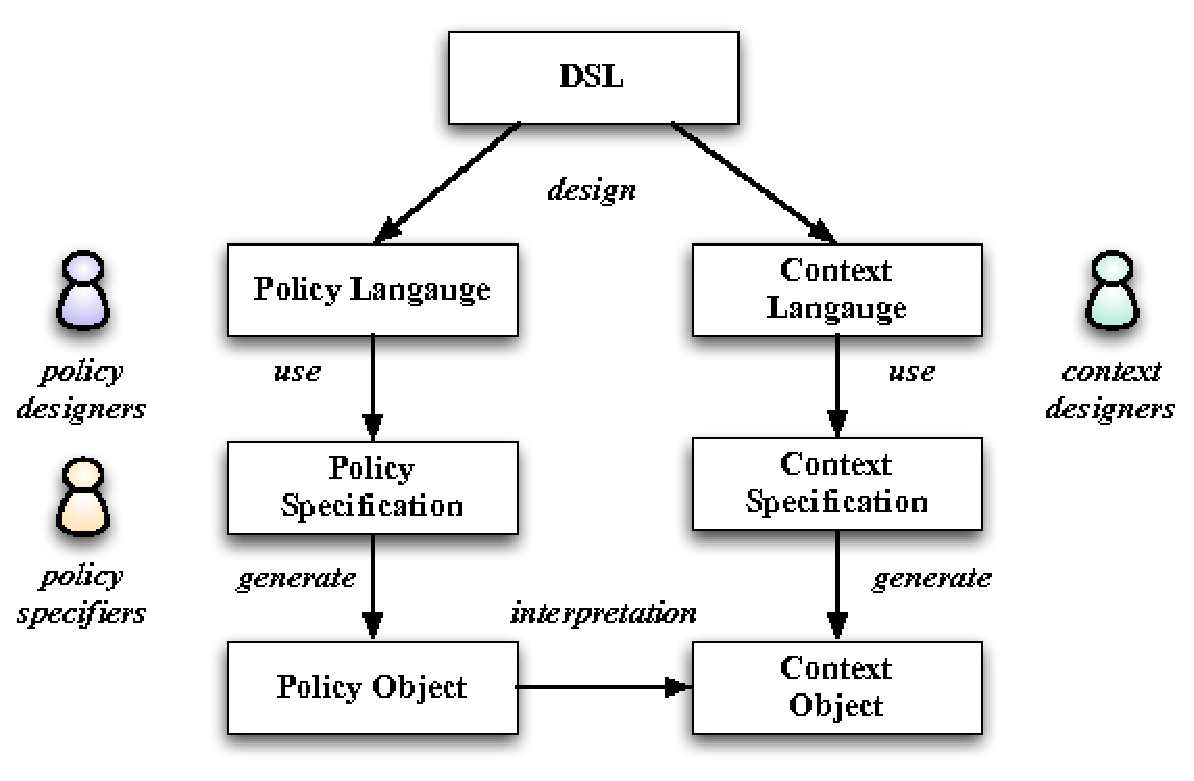
\includegraphics[width=2.4in]{players}
\begin{itemize}
\item<2-> \textit{DSL} --- Domain specific language
\item<3-> \textit{Policy Language} --- Language elements specific to \textit{policy}
\end{itemize}
\column{.5\textwidth}
\begin{itemize}
\item<4-> \textit{Context Language} --- Language elements specific to \textit{context}
\item<5-> \textit{Policy Specification} --- Actual specification of policy
\item<6-> \textit{Context Specification} --- Specification of context requirements
\item<7-> \textit{Policy Object} --- An object embodying policy created from the DSL
\item<8-> \textit{Context Object} --- An object containing context
\end{itemize}
\end{columns}
\end{frame}

\begin{frame}[t]
\frametitle{Design --- Use Cases}
\begin{columns}[t]
\column{.5\textwidth}
Use Cases:
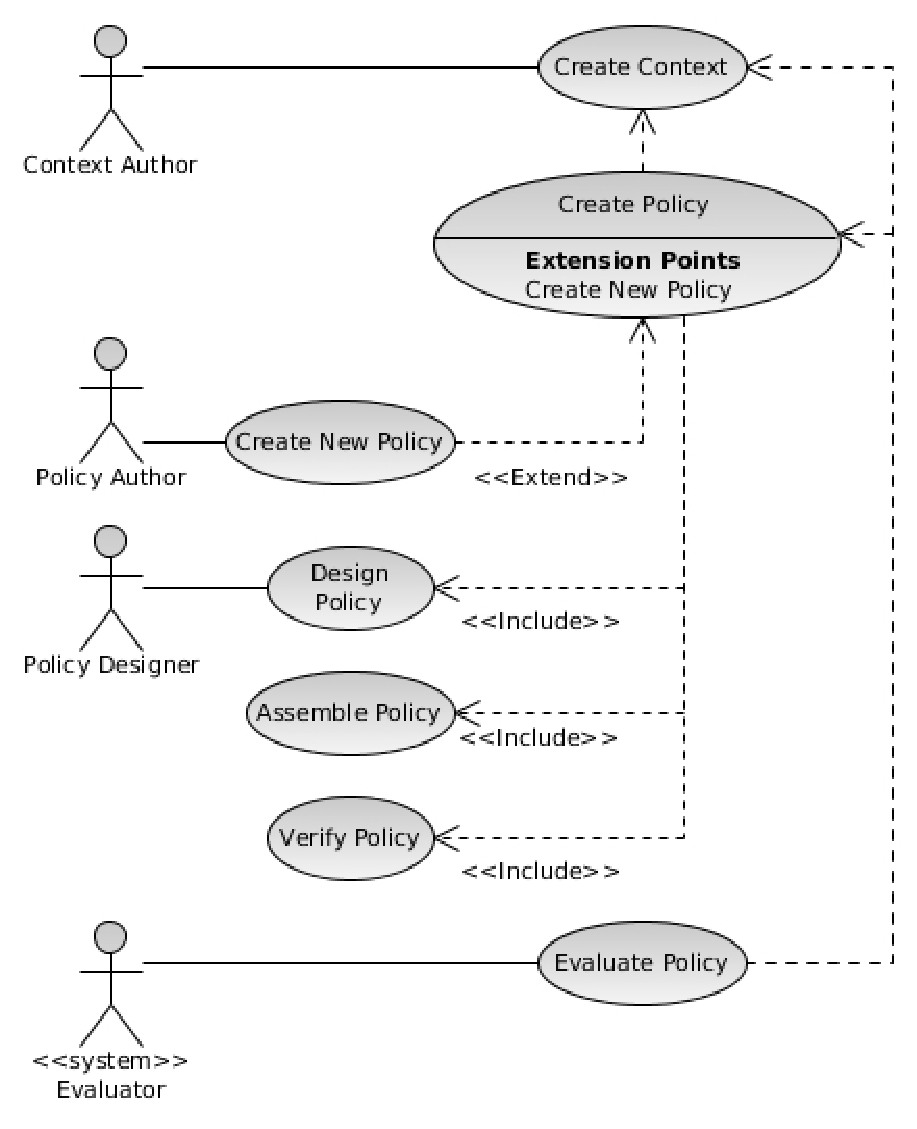
\includegraphics[width=2.3in]{use-cases}
\column{.5\textwidth}
\begin{itemize}
\item<2-> \textit{Create Context} --- Prior to creating a policy, the context in which that policy will be evaluated must be defined.
\item<3-> \textit{Create Policy} --- A designer creates a new type of policy, embodied by specific extension elements or semantic constraints over existing elements.  An author will use these to create an instance of a policy.
\item<4-> \textit{Evaluate Policy} --- The policy is evaluated with a context.
\end{itemize}
\end{columns}
\end{frame}

\begin{frame}[t]
\frametitle{Design --- Domain Model}
\begin{columns}[t]
\column{.5\textwidth}
Domain Model:
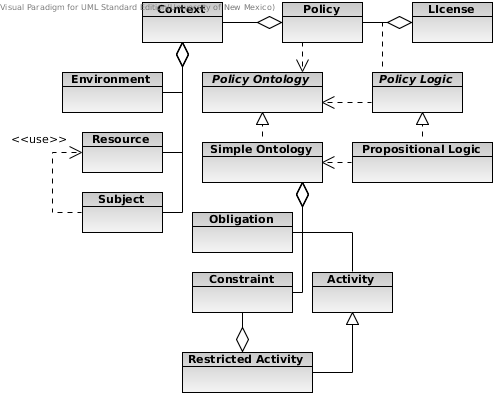
\includegraphics[width=2.3in]{ontology}
\column{.5\textwidth}
\pause
The \textit{Runtime} accesses and activates a \textit{policy} and manages a \textit{context} to which the policy is given a reference.
\newline
\newline
\pause
The \textit{context} has access to information about the \textit{environment}, \textit{resource} managed, and the \textit{subject} using the \textit{resource}. 
\newline
\newline
\pause
Interactions are described by specific \textit{usage semantics} embodied in the \textit{policy}.
\end{columns}
\end{frame}

\begin{frame}[t]
\frametitle{Design --- Usage Semantics}
\begin{columns}[t]
\column{.5\textwidth}
Usage Semantics:
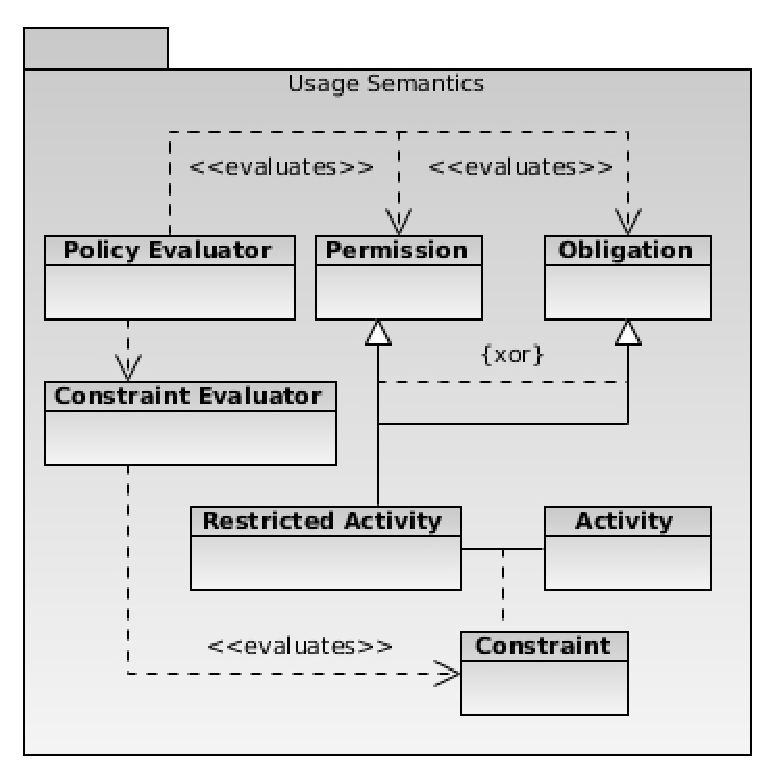
\includegraphics[width=2.3in]{usage-semantics}
\column{.5\textwidth}
\pause
A \textit{policy evaluator} examines and rectifies both \textit{permissions} and \textit{Obligations}.
\newline
\newline
\pause
A \textit{restricted activity} is a specialization of either a \textit{permission} or \textit{obligation}, and is associated with a specific \textit{activity}.
\newline
\newline
\pause
The association between an \textit{activity} and a \textit{restricted activity} is embodied by a \textit{constraint}, which is evaluated by a \textit{constraint evaluator}.
\end{columns}
\end{frame}

\section{Implementation}
\begin{frame}[t]
\frametitle{Implementation --- Lifecycle}
Typical DSL Lifecycle: \\
\begin{center}
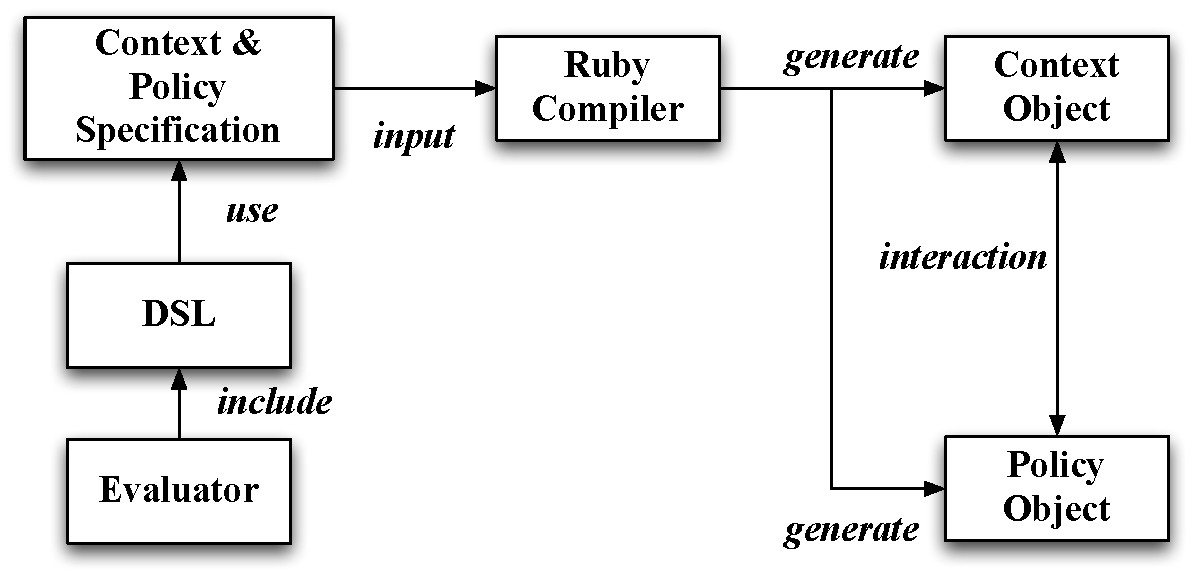
\includegraphics[width=4in]{DSL-usage}
\end{center}
\end{frame}

\begin{frame}[t]
\frametitle{Implementation --- Attributes}


%\begin{table*}[t]
%\caption{An example structure of context.}
\label{table:context}
\begin{center}
{\tiny
\begin{tabular}{|c|c|c|c|}
\hline
\multicolumn{4}{|c|}{ \bf Context}\\
\hline
{ \bf Entity} & {\bf Property ($p$)} & { \bf Domain ($D_p$)} & {\bf Functions ($F_p$)}\\
\hline
{Environment (E)} & OperatingSystem & \{Windows, OSX, SELinux\}&  equatable\\
                                                    & Device & \{Workstation, Handheld, Blackberry, Terminal\} & equatable \\
                                                    & SecurityDomain & \{ ABNet, SECNet, TELNet, OMNINet\} & comparable\\ 
\hline
{Subject (S)} & SecurityClearance & \{Top Secret, Secret, Confidential\} &  comparable\\
				      &Project & \{Zebra, Yuma, Lion\} & equatable\\
				       &Role & \{Alpha, Beta, Delta\} & equatable\\

\hline
 Resource(R) & SecurityClassification & \{ Top Secret, Secret, Confidential, Unclassified\} & comparable \\
\hline
\end{tabular}
}
\end{center}
{\small
{\bf Environment (E):} \\
Operating System $\rightarrow$  \{Windows, OSX, SELinux\} $\rightarrow$  equatable\\
Device $\rightarrow$  \{Workstation, Handheld, Blackberry, Terminal\} $\rightarrow$  equatable \\
Security Domain $\rightarrow$ \{ABNet, SECNet, TELNet, OMNINet\} $\rightarrow$ comparable \\
{\bf Subject(S):} \\
SecurityClearance $\rightarrow$ \{Top Secret, Secret, Confidential\} $\rightarrow$ comparable\\
Project $\rightarrow$ \{Zebra, Yuma, Lion\} $\rightarrow$ equatable\\
Role $\rightarrow$ \{Alpha, Beta, Delta\} $\rightarrow$ equatable\\
{\bf Resource(S):} \\
Classification $\rightarrow$ \{TopSecret, Secret, Confidential, Unclassified\} $\rightarrow$ comparable\\
}
\end{frame}

\begin{frame}[t]
\frametitle{Implementation --- Properties}
\lstinputlisting[]{content/code/policy/property_1.pol}
\end{frame}

\begin{frame}[t]
\frametitle{Implementation --- Properties}
\lstinputlisting[]{content/code/policy/property_2.pol}
\end{frame}

\begin{frame}[t]
\frametitle{Implementation --- Entity, Context}
\lstinputlisting[]{content/code/policy/entity.pol}
\pause
\lstinputlisting[]{content/code/policy/context.pol}
\end{frame}

\begin{frame}[t]
\frametitle{Implementation --- Activities, Constraints}
\lstinputlisting[]{content/code/policy/activity_1.pol}
\pause
\lstinputlisting[]{content/code/policy/activity_2.pol}
\end{frame}


\begin{frame}[t]
\frametitle{Implementation --- Policies}
\lstinputlisting[]{content/code/policy/policy_1.pol}
\pause
\lstinputlisting[]{content/code/policy/policy_2.pol}
\end{frame}

\begin{frame}[t]
\frametitle{Implementation - Interface}
\begin{itemize}
\item<2-> {\bf permissions?()}. Returns the set of permissions for a given policy.
\item<3-> {\bf obligations?(a)}. Returns the set of all obligations associated with a given permission. 
\item<4-> {\bf remaining\_obligations(a)}. Returns the set of remaining obligations for a given permission. 
\item<5-> {\bf remaining\_count(a)}. Returns the set of remaining count for a given permission. 
\item<6-> {\bf allowed?(a, ctx)}. A boolean function that returns {\em true/false} whether a given activity can be carried out under a given context. 
\item<7-> {\bf reset()}. Resets the policy by resetting its state. 
\end{itemize}
\end{frame}

\section{Application}
%%%%%%%%%%%%%%%%%%%%%%%%%%%%%%%%%%%%%%%%%%%%%
\begin{frame}[t]
    \frametitle{Application - CC REL}
    \begin{itemize}
        \item The Creative Commons Rights Expression Language
        \item RDFa (Resource Description Framework in attributes) for HTML
        Web pages and resources referenced therein
        \item XMP (Extensible Metadata Platform) for stand-alone media
        \item \texttt{http://wiki.creativecommons.org/CC\_REL}
    \end{itemize}
\end{frame}

%%%%%%%%%%%%%%%%%%%%%%%%%%%%%%%%%%%%%%%%%%%%%
\begin{frame}[fragile]
\frametitle{Application - RDFa in HTML}
        \begin{itemize}
            \item Can simply associate web content with a CC license:
        \end{itemize}
\lstinputlisting[language=HTML]{listings/RDFaExample.html}
        \begin{itemize}
            \item But what are the semantics of \url{http://creativecommons.org/licenses/by/3.0/}?
        \end{itemize}
\end{frame}

%%%%%%%%%%%%%%%%%%%%%%%%%%%%%%%%%%%%%%%%%%%%%
\begin{frame}[t]
\frametitle{Application - License Deed Webpage}
        \begin{itemize}
            %\item Looking at license URL as rendered
            %in browser, it's not obvious how a machine could
            %derive semantics:
            \item Can a machine derive this page's semantics?
        \end{itemize}
        \begin{center}
            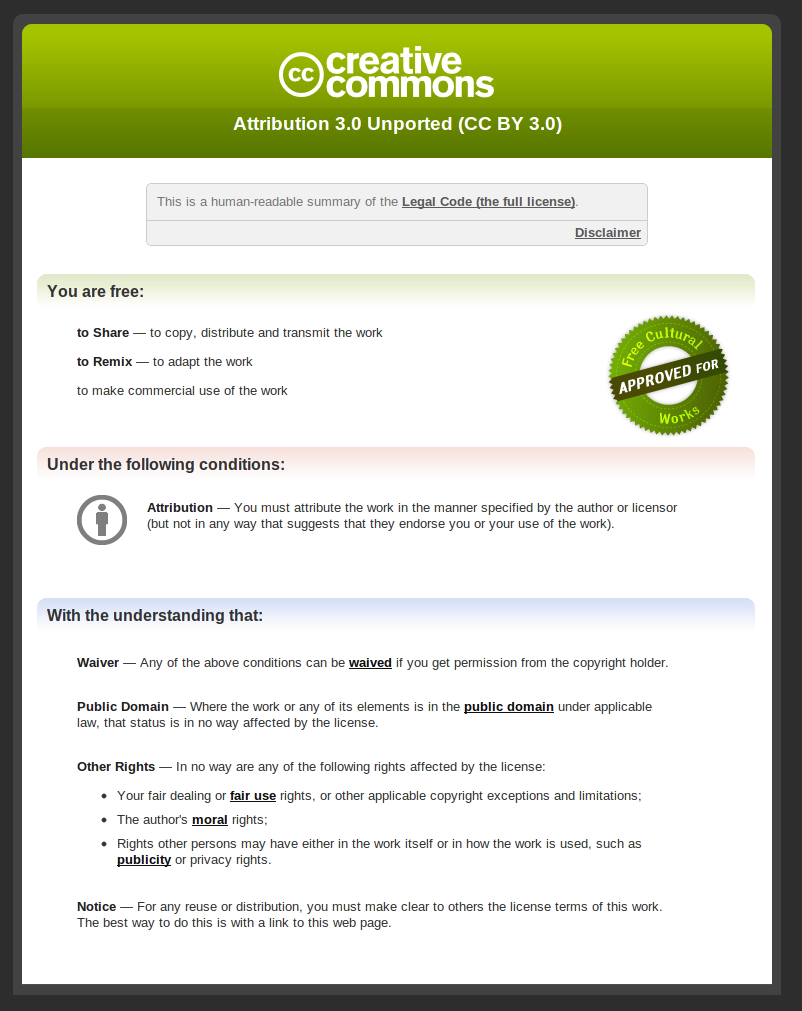
\includegraphics[height=0.8\textheight]{resources/cc/cc-deed-rendered-in-browser.png}
        \end{center}
\end{frame}

%%%%%%%%%%%%%%%%%%%%%%%%%%%%%%%%%%%%%%%%%%%%%
\begin{frame}[fragile]
\frametitle{Application - RDF Embedded}
        \begin{itemize}
            \item The previous webpage contains the following embedded RDF:
        \end{itemize}
\lstinputlisting[language=HTML]{listings/CC-deed-embeded-RDF.xml}
        \begin{itemize}
            \item From this, a machine can determine that this license:
            \begin{itemize}
                \item Permits:
                    \begin{itemize}
                        \item \texttt{\#DerivativeWorks}, \texttt{\#Distribution}, \texttt{\#Reproduction}
                    \end{itemize}
                \item Requires:
                    \begin{itemize}
                        \item \texttt{\#Attribution}, \texttt{\#Notice}
                    \end{itemize}
            \end{itemize}
            \item However, what do these things mean?  How are they implemented?
        \end{itemize}
\end{frame}

%%%%%%%%%%%%%%%%%%%%%%%%%%%%%%%%%%%%%%%%%%%%%
\begin{frame}[t]
\frametitle{Application - RDFa Embedded}
        \begin{itemize}
            \item In addition to the RDF shown on previous slide, CC License Deeds also have embedded RDFa
            \item You can see that a machine can parse this data with something
            like the RDFa Distiller and Parser Tool:
        \end{itemize}
        \begin{center}
            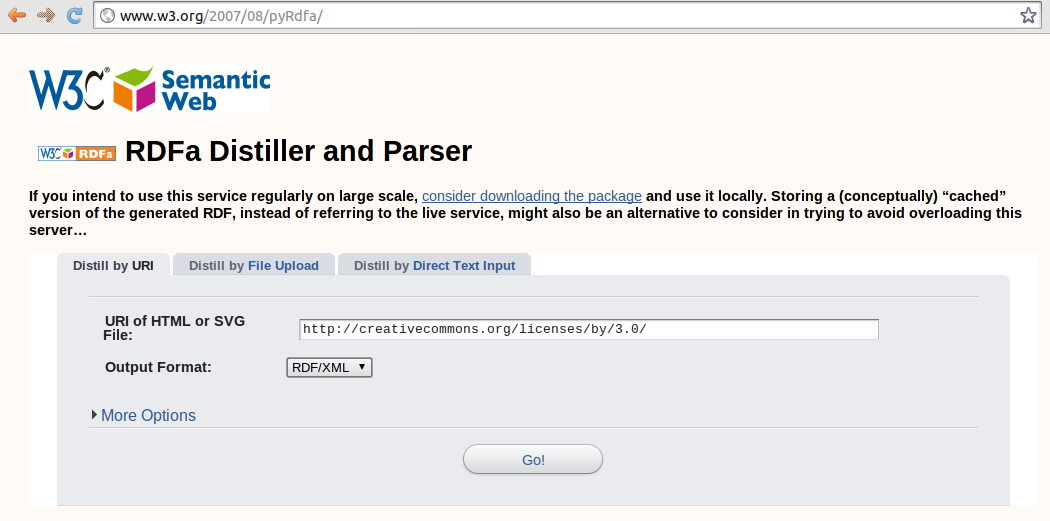
\includegraphics[width=0.8\textwidth]{resources/RDF/RDFa-distiller.png}
        \end{center}
\end{frame}


%%%%%%%%%%%%%%%%%%%%%%%%%%%%%%%%%%%%%%%%%%%%%
\begin{frame}[fragile]
\frametitle{Application - RDFa Distiller}
\lstinputlisting[language=HTML]{listings/RDF-from-RDFa-distiller.xml}
\end{frame}

%%%%%%%%%%%%%%%%%%%%%%%%%%%%%%%%%%%%%%%%%%%%%
\begin{frame}[t]
\frametitle{Application - CC RDF Schema}
        \begin{itemize}
            \item License RDF(a) references \texttt{\#DerivativeWorks}, etc.,
            in the CC namespace that's defined by a schema that's
            human-readable and machine-readable RDF.
            \item But... how immediately machine actionable is this schema?
            \item Partial screenshot below:
        \end{itemize}
        \begin{center}
            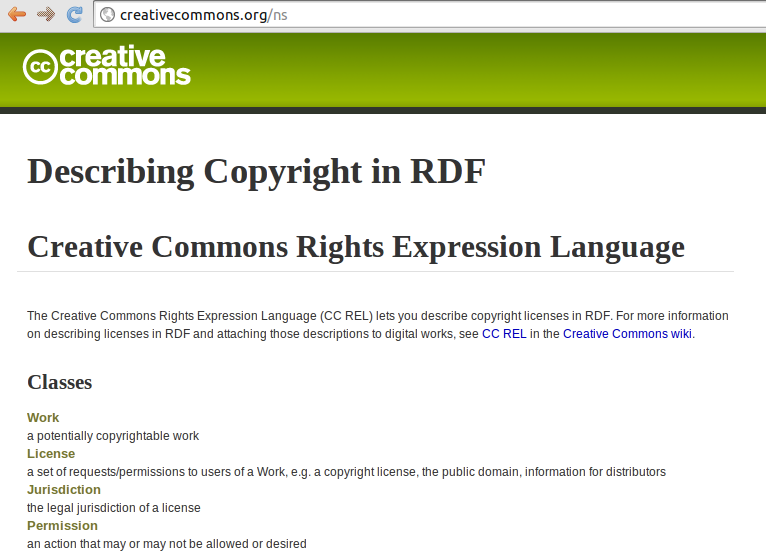
\includegraphics[width=0.4\textwidth]{resources/cc/schema-screenshot-partial.png}
        \end{center}
        \begin{itemize}
            \item We would like to investigate replacing or augmenting RDF(a)
            in the license deed with a license that's described with our DSL
        \end{itemize}
\end{frame}

%%%%%%%%%%%%%%%%%%%%%%%%%%%%%%%%%%%%%%%%%%%%%
\begin{frame}[t]
\frametitle{Application - DSL}
    \begin{itemize}
        \item By investigating replacing the contents of a license like
        \url{http://creativecommons.org/licenses/by/3.0/} with something that
        expresses the license in terms our DSL, we hope to:
        \begin{itemize}
            \item Maintain equivalent license semantics
            \item Express the semantics in a form that is easier for humans to read and write
            \item Enable a machine to more directly execute the license and reason over it
        \end{itemize}
    \end{itemize}
\end{frame}

\begin{frame}[t]
\frametitle{Conclusions}
\pause
\begin{itemize}
\item Internal DSLs are convenient, but probably not appropriate for real systems
\pause
\item Overall we like the DSL but could do without some of the Ruby cruft (e.g. \textbf{do...end}, etc.)
\pause
\item Application and Optimization
\end{itemize}
\pause
%Questions?
%\newline
%\newline
%Chris Lamb: cclamb@ece.unm.edu \\
%Pramod Jamkhedkar: pramod54@ece.unm.edu \\
%Greg Heileman: heileman@ece.unm.edu \\
%Mathew P. Bohnsack: bohnsack@gmail.com \\
%Viswanath Nandina: vishu@ece.unm.edu
\end{frame}

\end{document}

